%  LaTeX support: latex@mdpi.com 
%  For support, please attach all files needed for compiling as well as the log file, and specify your operating system, LaTeX version, and LaTeX editor.

%=================================================================
\documentclass[aerospace,article,submit,moreauthors,dvi2pdf]{Definitions/mdpi} 

% For posting an early version of this manuscript as a preprint, you may use "preprints" as the journal and change "submit" to "accept". The document class line would be, e.g., \documentclass[preprints,article,accept,moreauthors,pdftex]{mdpi}. This is especially recommended for submission to arXiv, where line numbers should be removed before posting. For preprints.org, the editorial staff will make this change immediately prior to posting.

%--------------------
% Class Options:
%--------------------
%----------
% journal
%----------
% Choose between the following MDPI journals:
% acoustics, actuators, addictions, admsci, adolescents, aerospace, agriculture, agriengineering, agronomy, ai, algorithms, allergies, analytica, animals, antibiotics, antibodies, antioxidants, appliedchem, applmech, applmicrobiol, applnano, applsci, arts, asi, atmosphere, atoms, audiolres, automation, axioms, batteries, bdcc, behavsci, beverages, biochem, bioengineering, biologics, biology, biomechanics, biomedicines, biomedinformatics, biomimetics, biomolecules, biophysica, biosensors, biotech, birds, bloods, brainsci, buildings, businesses, cancers, carbon, cardiogenetics, catalysts, cells, ceramics, challenges, chemengineering, chemistry, chemosensors, chemproc, children, civileng, cleantechnol, climate, clinpract, clockssleep, cmd, coatings, colloids, compounds, computation, computers, condensedmatter, conservation, constrmater, cosmetics, crops, cryptography, crystals, curroncol, cyber, dairy, data, dentistry, dermato, dermatopathology, designs, diabetology, diagnostics, digital, disabilities, diseases, diversity, dna, drones, dynamics, earth, ebj, ecologies, econometrics, economies, education, ejihpe, electricity, electrochem, electronicmat, electronics, encyclopedia, endocrines, energies, eng, engproc, entropy, environments, environsciproc, epidemiologia, epigenomes, fermentation, fibers, fire, fishes, fluids, foods, forecasting, forensicsci, forests, fractalfract, fuels, futureinternet, futuretransp, futurepharmacol, futurephys, galaxies, games, gases, gastroent, gastrointestdisord, gels, genealogy, genes, geographies, geohazards, geomatics, geosciences, geotechnics, geriatrics, hazardousmatters, healthcare, hearts, hemato, heritage, highthroughput, histories, horticulturae, humanities, hydrogen, hydrology, hygiene, idr, ijerph, ijfs, ijgi, ijms, ijns, ijtm, ijtpp, immuno, informatics, information, infrastructures, inorganics, insects, instruments, inventions, iot, j, jcdd, jcm, jcp, jcs, jdb, jfb, jfmk, jimaging, jintelligence, jlpea, jmmp, jmp, jmse, jne, jnt, jof, joitmc, jor, journalmedia, jox, jpm, jrfm, jsan, jtaer, jzbg, kidney, land, languages, laws, life, liquids, literature, livers, logistics, lubricants, machines, macromol, magnetism, magnetochemistry, make, marinedrugs, materials, materproc, mathematics, mca, measurements, medicina, medicines, medsci, membranes, metabolites, metals, metrology, micro, microarrays, microbiolres, micromachines, microorganisms, minerals, mining, modelling, molbank, molecules, mps, mti, nanoenergyadv, nanomanufacturing, nanomaterials, ncrna, network, neuroglia, neurolint, neurosci, nitrogen, notspecified, nri, nursrep, nutrients, obesities, oceans, ohbm, onco, oncopathology, optics, oral, organics, osteology, oxygen, parasites, parasitologia, particles, pathogens, pathophysiology, pediatrrep, pharmaceuticals, pharmaceutics, pharmacy, philosophies, photochem, photonics, physchem, physics, physiolsci, plants, plasma, pollutants, polymers, polysaccharides, proceedings, processes, prosthesis, proteomes, psych, psychiatryint, publications, quantumrep, quaternary, qubs, radiation, reactions, recycling, regeneration, religions, remotesensing, reports, reprodmed, resources, risks, robotics, safety, sci, scipharm, sensors, separations, sexes, signals, sinusitis, smartcities, sna, societies, socsci, soilsystems, solids, sports, standards, stats, stresses, surfaces, surgeries, suschem, sustainability, symmetry, systems, taxonomy, technologies, telecom, textiles, thermo, tourismhosp, toxics, toxins, transplantology, traumas, tropicalmed, universe, urbansci, uro, vaccines, vehicles, vetsci, vibration, viruses, vision, water, wevj, women, world 

%---------
% article
%---------
% The default type of manuscript is "article", but can be replaced by: 
% abstract, addendum, article, book, bookreview, briefreport, casereport, comment, commentary, communication, conferenceproceedings, correction, conferencereport, entry, expressionofconcern, extendedabstract, datadescriptor, editorial, essay, erratum, hypothesis, interestingimage, obituary, opinion, projectreport, reply, retraction, review, perspective, protocol, shortnote, studyprotocol, systematicreview, supfile, technicalnote, viewpoint, guidelines, registeredreport, tutorial
% supfile = supplementary materials

%----------
% submit
%----------
% The class option "submit" will be changed to "accept" by the Editorial Office when the paper is accepted. This will only make changes to the frontpage (e.g., the logo of the journal will get visible), the headings, and the copyright information. Also, line numbering will be removed. Journal info and pagination for accepted papers will also be assigned by the Editorial Office.

%------------------
% moreauthors
%------------------
% If there is only one author the class option oneauthor should be used. Otherwise use the class option moreauthors.

%---------
% pdftex
%---------
% The option pdftex is for use with pdfLaTeX. If eps figures are used, remove the option pdftex and use LaTeX and dvi2pdf.

%=================================================================
\graphicspath{{figures/}}
% MDPI internal commands
\firstpage{1} 
\makeatletter 
\setcounter{page}{\@firstpage} 
\makeatother
\pubvolume{1}
\issuenum{1}
\articlenumber{0}
\pubyear{2021}
\copyrightyear{2020}
%\externaleditor{Academic Editor: Firstname Lastname} % For journal Automation, please change Academic Editor to "Communicated by"
\datereceived{} 
\dateaccepted{} 
\datepublished{} 
\hreflink{https://doi.org/} % If needed use \linebreak
%------------------------------------------------------------------
% The following line should be uncommented if the LaTeX file is uploaded to arXiv.org
%\pdfoutput=1

%=================================================================
\usepackage{arydshln}
 \usepackage{multirow}
 \usepackage{siunitx}
 \usepackage{wasysym}
% Add packages and commands here. The following packages are loaded in our class file: fontenc, inputenc, calc, indentfirst, fancyhdr, graphicx, epstopdf, lastpage, ifthen, lineno, float, amsmath, setspace, enumitem, mathpazo, booktabs, titlesec, etoolbox, tabto, xcolor, soul, multirow, microtype, tikz, totcount, changepage, paracol, attrib, upgreek, cleveref, amsthm, hyphenat, natbib, hyperref, footmisc, url, geometry, newfloat, caption
%=================================================================
%% Please use the following mathematics environments: Theorem, Lemma, Corollary, Proposition, Characterization, Property, Problem, Example, ExamplesandDefinitions, Hypothesis, Remark, Definition, Notation, Assumption
%% For proofs, please use the proof environment (the amsthm package is loaded by the MDPI class).

%=================================================================
% Full title of the paper (Capitalized)
\Title{Design of a Low Cost Air Bearing Testbed for Nano CMG Manoeuvres }

% MDPI internal command: Title for citation in the left column
\TitleCitation{Title}

% Author Orchid ID: enter ID or remove command
\newcommand{\orcidauthorA}{0000-0003-3114-3330} % Add \orcidA{} behind the author's name
%\newcommand{\orcidauthorB}{0000-0000-0000-000X} % Add \orcidB{} behind the author's name

% Authors, for the paper (add full first names)
\Author{Charalampos Papakonstantinou $^{1,\dagger}$*\orcidA{},Georgios Moraitis $^{2,\dagger}$, Vaios J. Lappas $^{3}$ and Vassilis Kostopoulos $^{4,\dagger}$}

% MDPI internal command: Authors, for metadata in PDF
\AuthorNames{Charalampos Papakonstantinou, Georgios Moraitis, Vaios J. Lappas and Vassilis Kostopoulos}

% MDPI internal command: Authors, for citation in the left column
\AuthorCitation{Papakonstantinou, C.; Moraitis, G.; Lappas, V.; Kostopoulos, V.}
% If this is a Chicago style journal: Lastname, Firstname, Firstname Lastname, and Firstname Lastname.

% Affiliations / Addresses (Add [1] after \address if there is only one affiliation.)
\address{%
$^{1}$ \quad Ph.D Student, Department of Mechanical Engineering and Aeronautics;  c\_papakonstantinou@upnet.gr\\
$^{2}$ \quad Ph.D Student, Department of Mechanical Engineering and Aeronautics, georgios.moraitis@upnet.gr\\
$^{3}$ \quad Department of Aerospace Science and Technology, National Kapodistrian University of Athens, Athens, Greece, 10679; vlappas@upatras.gr\\
$^{4}$ \quad Professor, Department of Mechanical Engineering and Aeronautics, Director of Applied Mechanics and Vibrations Laboratory; kostopoulos@upatras.gr\\
}

% Contact information of the corresponding author
\corres{Correspondence: c\_papakonstantinou@upnet.gr;
Tel.: +306989124655 +0000-0003-3114-3330 (C.P.)}

% Current address and/or shared authorship
\firstnote{University of Patras, Rio, Greece, 26504} 
% \secondnote{These authors contributed equally to this work.}
% The commands \thirdnote{} till \eighthnote{} are available for further notes

%\simplesumm{} % Simple summary

%\conference{} % An extended version of a conference paper

% Abstract (Do not insert blank lines, i.e. \\) 
\abstract{In this paper, a low cost, miniature spacecraft attitude control simulator is presented for testing miniature actuators such as Nano Control Moment Gyroscopes (CMGs) for simple manoeuvres. The experimental setup is composed by the attitude control system (ACS) that mainly consists of a four CMG cluster in a pyramid configuration and a custom made air bearing. The one degree of freedom (DoF) air bearing is fabricated to reproduce the frictionless conditions of a nano-satellite in orbit. The ACS is made exclusively using low cost commercial-off-the-shelf (COTS) components whilst the air bearing is made by 3D printed parts. Both hardware and software implementations are described in detail and the performance of the developed simulator is evaluated by two manoeuvre experiments. Despite the manufacturing imperfections, the ACS is capable of providing higher angular velocities than previously presented in the literature while following the theoretical/simulation data. The results indicate that it is possible to manufacture a lightweight actuator of small dimensions using COTS components to demonstrate the operation of an agile nano-satellite. Any deviations from the theoretical values are addressed and several improvements are discussed to further enhance the performance of the air bearing testing platform.}

% Keywords
\keyword{Spacecraft attitude control simulator, control moment gyroscope cluster, pyramid configuration, air bearing, agile manoeuvring} 

% The fields PACS, MSC, and JEL may be left empty or commented out if not applicable
%\PACS{J0101}
%\MSC{}
%\JEL{}

%%%%%%%%%%%%%%%%%%%%%%%%%%%%%%%%%%%%%%%%%%
% Only for the journal Diversity
%\LSID{\url{http://}}

%%%%%%%%%%%%%%%%%%%%%%%%%%%%%%%%%%%%%%%%%%
% Only for the journal Applied Sciences:
%\featuredapplication{Authors are encouraged to provide a concise description of the specific application or a potential application of the work. This section is not mandatory.}
%%%%%%%%%%%%%%%%%%%%%%%%%%%%%%%%%%%%%%%%%%

%%%%%%%%%%%%%%%%%%%%%%%%%%%%%%%%%%%%%%%%%%
% Only for the journal Data:
%\dataset{DOI number or link to the deposited data set in cases where the data set is published or set to be published separately. If the data set is submitted and will be published as a supplement to this paper in the journal Data, this field will be filled by the editors of the journal. In this case, please make sure to submit the data set as a supplement when entering your manuscript into our manuscript editorial system.}

%\datasetlicense{license under which the data set is made available (CC0, CC-BY, CC-BY-SA, CC-BY-NC, etc.)}

%%%%%%%%%%%%%%%%%%%%%%%%%%%%%%%%%%%%%%%%%%
% Only for the journal Toxins
%\keycontribution{The breakthroughs or highlights of the manuscript. Authors can write one or two sentences to describe the most important part of the paper.}

%%%%%%%%%%%%%%%%%%%%%%%%%%%%%%%%%%%%%%%%%%
% Only for the journal Encyclopedia
%\encyclopediadef{Instead of the abstract}
%\entrylink{The Link to this entry published on the encyclopedia platform.}
%%%%%%%%%%%%%%%%%%%%%%%%%%%%%%%%%%%%%%%%%%

\begin{document}
%%%%%%%%%%%%%%%%%%%%%%%%%%%%%%%%%%%%%%%%%%
% \setcounter{section}{-1} %% Remove this when starting to work on the template.

\section{Introduction}

With over 350 nano-satellites to have been set in orbit between 2020 and 2021 \cite{nanosats}, it is evident that nano-satellites are in the front-line of the space industry. Their light weight and the low manufacturing cost allows for technological and scientific principles to be demonstrated in a rapid and effective way. Even though, it is vital to perform tests on ground-based conditions before a spacecraft is set in orbit to ensure the success of a space mission that takes place in micro-gravity conditions, simulating the space environment in a laboratory is a complex task. Ground simulations of the attitude control system (ACS), one of the most challenging subsystems of the satellite, are commonly achieved using air bearings because they establish a thin film of air capable of supporting the experimental equipment in a near frictionless way. Air bearings are usually divided in three main types. Planar air bearings allow only translational movements while rotational air bearings allow the rotation around at least one of the roll, pitch or yaw axis. On the other hand, the combinational air bearings offer enhanced capabilities by moving the ACS in six or less degrees of freedom (DoF). 
A wide range of air-bearing-based spacecraft simulators has been developed. The most recent of them are manufactured for nano and micro-satellite testing and they are presented below. 
% An attitude control simulator based on a spherical air bearing has been presented in \ref{2} for mini-satellite testing, based on a PC104 type Intel mobile Pentium 266MHz on board computer. Three flywheels are used for attitude control and an inertial measurement unit (IMU) manufactured by Crossbow Technology Inc. is used for attitude determination.
% A second mini-satellite attitude simulator has been manufactured by the School of Aerospace Engineering at the Georgia Institute of Technology. However, the new platform is controlled by an Intel Pentium III 750MHz processor that controls eight gas thrusters and four variable speed CMGs \cite{1}.
% The University of Michigan has developed a three-axis testbed in dumbbell configuration allowing the unrestricted motion about the yaw and the roll axis \cite{55}. It is based on a Quanser Consulting processor and it is equipped with a set of six reaction wheels. 

The Space Vehicle Control Group of the University of Surrey's has also used an one DoF air bearing table to demonstrate the benefits of the miniaturization of control moment gyroscopes (CMGs). Four CMGs are used in pyramid configuration controlled by a Siemens 8 bit C515 microcontroller while an inertial measurement unit (IMU) by Crossbow Technology Inc. is exploited to measure the angular rate of the platform \cite{lappasthesis}. Utilizing all four CMGs for a manoeuvre about the vertical axis, the cluster is capable of rotating the platform with a maximum angular velocity of 8.41deg/s.
% Two separate spherical air bearing platforms have been developed by the Department of Aerospace \& Ocean Engineering at Virginia Polytechnic Institute \& State University \cite{28}. The first is called Whorl-I and it is in tabletop configuration allowing a $\pm$5 deg rotation about the horizontal plane. The second is called Whorl-II is a dumbbell style air bearing that restrict the motion to $\pm$30 deg only about pitch axis. Both spacecraft control simulators are based on the PC/104+ form-factor. Three-axis flywheels either on momentum or reaction mode along with compressed air thrusters and CMGs are used for attitude control. 
% A custom-made air bearing is presented in \cite{32} based on a 16-bit SAB80C166 RISC microcontroller. The testbed is a round-shaped table with an external diameter of 76 cm, supporting a nominal load of 80 kg. An electronic compass, inclinometers and a sun sensor are used for  attitude determination whilst three flywheels control the orientation of the simulator.
% --
Another tabletop-style, hemispherical air bearing is described in \cite{7}. A circular disk with 30 cm of diameter and thickness 10 mm is developed for testing the behaviour of nano-satellites, up to 2U CubeSats. The testbed is based on an Arduino Mega 2560 board and it is equipped with a 9 DoF Sparkfun IMU along with three reaction wheels for attitude determination and control.
% --
An extremely simple apparatus with cost of less than \$20 made exclusively for educational purposes is presented in \cite{12}. It consists of an air bearing made by casting polyester resin and a billiard ball that is used for rotational motion and precession demonstrations.
% --
The Naval Postgraduate School has also designed an air bearing platform for testing the ACS of the micro-satellite NPSAT1 \cite{3}.  The air bearing allows a maximum tilt angle of 32 deg about the horizontal plane and a 360 deg motion about the vertical axis. The testbed is designed to hold up to 82 kg requiring approximately 24 psi of air pressure supply.
% --
Another attitude simulator, called CubeTAS is developed for nano-satellite testing. It is based on PC-104 form factor and an ARM9 processor  \cite{14}. The bottom part of the air bearing is a hemisphere with diameter of 250mm and the rotational motion is limited to $\pm$50 deg about the horizontal plane. An IMU and three reaction wheels are used for attitude determination and control while a Helmholtz cage is installed around the platform to simulate the Earth's magnetic field. 
% --
York University has presented another nano-satellite attitude simulator which makes use of a commercial-off-the-shelf (COTS) air bearing designed by Nelson Air \cite{27}. The testbed is based on a Linuxstamp II an it is equipped with an ADIS16364 six-DoF IMU and three orthogonally mounted reaction wheels.
% --
A cubesat attitude control simulator has been developed by the Massachusetts Institute of Technology based on a tabletop air bearing with diameter of 12.4 cm \cite{58}. Four flywheels operating either in reaction or momentum wheel mode are used while the ADIS 16365 IMU made by Analog Devices and the three-axial MicroMag3 made by PNI Corporation are the sensors of the system. The platform is controlled by two Arduino Mega boards.
% --
Another tabletop-style aerostatic bearing is developed by the Instituto Tecnológico de Aeronáutica of Brazil \cite{39}. It consists of three-axial gyroscopes and a set of three orthogonally installed reaction wheels that can provide a maximum manoeuvring speed of 0.33 deg/s.
% --
An air bearing with a porous carbon surface has been used by the Aerospace Engineering Department of the United States Naval Academy \cite{15} for micro-satellite testing. The tests include a 11.3 kg platform, based on an Arduino processor, an Adafruit 9-DoF IMU for attitude determination and a set of four reaction wheels for controlling orientation of the platform. The simulator and the actuators are designed to follow the requirement of a desired agility of 4 deg/s.
% --
Another air bearing in tabletop configuration that makes use of four reaction wheels and an AHRS sensor has been developed by the Department of Mechanical Engineering of University of Isfahan for testing a 40 kg platform \cite{21}.
% --
An attitude control testbed for cubesats has been built by the Virginia Polytechnic Institute and State University using COTS components \cite{13}. A tabletop-style air bearing manufactured by Space Electronics Inc. is used and the platform is controlled by a Beaglebone Black - Rev C board.  The VN-100 IMU/AHRS by VectorNav which embeds a three-axial magnetometer, accelerometer and gyroscope along with a barometric pressure sensor determines the attitude of the testbed. No actuators for attitude control are present on the simulator.
% --
A cubesat and nano-satellite simulator is presented in \cite{44}. A PLA 3D printed sphere encloses three reaction wheels, two perpendicular magnetorquers, an EZ-COMPASS-4 and a Sparkfun MPU-9150 for attitude control and determination.
Both sensors and actuators are controlled by a Raspberry PI 2 Model B board. Three distinct experiments were performed each one for every axis demonstrating a maximum angular velocity of less than 2 deg/s. 
 % --
 The Laboratory of Application and Innovation in Aerospace Science of the University of Brasília has manufactured a nano-satellite attitude simulator that consists of a custom made tabletop air bearing that limits the motion to $\pm$45 deg about the horizontal plane \cite{29}. An ATMEGA8 is the main computer of the testbed, an ADIS16400 IMU controls determines its orientation and there are no actuators on the platform for attitude control.
% --
Another attitude simulator for testing nano-satellite missions in low Earth orbit is presented in \cite{37}. The facility is capable of simulating both the light coming from the Sun and the Earth's magnetic field through COTS LED Studio and Helmholtz cage. The tabletop-style air bearing used has been made by Serviciencia and the platform is based on an Arduino Due board. The platform is equipped with magnetometer and a monochromatic CMOS camera that is used as a sun sensor while a custom monocular metrology vision system is also implemented for ground-truth attitude determination. With a total cost of less than 20k euros, the attitude simulator does not embed any actuators for attitude control.
% --
A 3D printed air bearing has been manufactured by Aalto University \cite{34}. The air bearing is made of PLA and two hollow hemispheres that connect through latching pieces form a full sphere that consists the rotor of the system. Directional air nozzles compensate for the disturbances produced by fabrication imperfections. A visual tracking system based on OpenCV library is used for torque measurements by calculating the angular velocity of the rotor through fixed markings on it.

It is evident that CMGs have not been commonly used in spacecraft attitude control simulators even though it is proven that they offer enhanced torque capabilities that meet the manoeuvring requirements of agile satellites \cite{SMCS, lappasthesis}. Reaction and momentum wheels can be widely found because they are affordable and it is easier to make since they use less moving parts compared to CMGs. In this paper, a simple and affordable approach is presented to fabricate a four CMG cluster in pyramid configuration using COTS components. A custom-made 3D printed air bearing that provides one rotational DoF about the vertical axis is also designed for testing. The experimental results follow the theoretical values and they confirm that it is feasible to demonstrate high manoeuvring capabilities using COTS components. 
 
 
%%%%%%%%%%%%%%%%%%%%%%%%%%%%%%%%%%%%%%%%%%
\section{System Overview}
The objective in the work presented is the development and evaluation of a 4-CMG pyramid cluster to be used for attitude control. The system should be designed to fit into a nano-satellite with a maximum mass value of under 2 kg while remaining at a reasonable cost. Moreover, specific manoeuvrability criteria have to be followed as described in the "Sizing" section. 

The developed Attitude Control System (ACS) is composed by the actuators and the electronic components that are mounted in a hemispherical structure in tabletop configuration. The main parts of the ACS are divided in hardware and software as presented below.
\subsection{Hardware}
All electronics are mounted on top of a 3D printed ABS rectangle plate with a hemispherical base while the total size of the platform with the CMGs employed is 17.8 cm $\times$ 17.8 cm $\times$ 18.3 cm. The 3D CAD model is shown along with the experimental setup in Figure~\ref{fig:myACS}a and Figure~\ref{fig:myACS}b respectively.

\begin{figure}[H]
\includegraphics[width=10.5cm]{cadvsmyacs.jpg}
\caption{ACS on hemispherical 3D printed platform. \textbf{a}) CAD model and \textbf{b}) Hardware setup \label{fig:myACS}}
\end{figure}

The parts that compose the ACS hardware are the main perfboard along with the microcontroller and the Inertial Measurement Unit (IMU), the battery and the four CMGs. The location of the equipment on the platform has been as symmetric as possible.

\begin{specialtable}[H] 
\caption{\label{table:componentsweight} Components Weight}
%%% \tablesize{} %% You can specify the fontsize here, e.g., \tablesize{\footnotesize}. If commented out \small will be used.
\begin{tabular}{lcc}
\toprule
\textbf{Component}  & \textbf{Units} & \textbf{Total Mass, g}   \\
\midrule
Gimbal DC motor &   4 &  42\\
Flywheel DC motor& 4 & 38\\
Flywheel disk & 4 & 52\\
Slip Ring     & 4 & 68\\
Encoder       & 8 &  8   \\
Battery        & 1 & 47\\
Perfboard with electronics  &1& 130 \\
Screws &12 & 55.2  \\
3D printed CMG parts &&138  \\
3D printed tabletop base && 163.67\\ % tabletop=(rectangle + ball )1=12.27+51.4
Other (wires, soldering material, LEDs etc.) && 20.93\\
Total            & & 762.8 g  \\
\bottomrule
\end{tabular}
\end{specialtable}


\subsubsection{CMGs}
A 4-CMG cluster in pyramid configuration is used for the attitude control of the platform. The main parts of the cluster are the eight micro DC motors. Four Pololu 3058 motors are used to implement the gimbals while four Pololu 3082 motors are used as flywheels. The gear ratio of the gimbal and flywheel motors , $g_r$, equals to 1006:1 and 5:1 respectively. A magnetic encoder is placed on the shaft of every motor. Each encoder is a dual-channel Hall Effect sensor board in combination with a 6-pole magnetic disc. The resolution they provide is 12 counts per revolution of the motor shaft and it can be converted in counts per revolution of the gearbox output shaft, $cpr_g$, through the following equation: 

\begin{equation}
cpr_{g}=12\cdot g_r
\end{equation}
The angle accuracy in degrees, $acc$, can be measured for each type of motor by:

\begin{equation}
acc=\frac{360}{cpr_{g}}
\end{equation}
Table~\ref{table:components} presents the details of the motors used.
\begin{specialtable}[H] 
\caption{\label{table:components} DC Motors Details}
%%% \tablesize{} %% You can specify the fontsize here, e.g., \tablesize{\footnotesize}. If commented out \small will be used.
\begin{tabular}{lccc}
\toprule
\textbf{Component}  & $g_r$ & $acc$ & \textbf{No load speed}    \\
\midrule
Gimbal DC & 1006:1 &0.0298 deg & 13 rpm \\
Flywheel DC   & 5:1 &6 deg & 6500 rpm\\
\bottomrule
\end{tabular}
\end{specialtable}

\subsubsection{Perfboard}
To enable a full 360 deg rotation about the gimbal axis for each CMG, the 6-Wire SRC022 slip ring by Adafruit is used. The motors nominal voltage is 6 V.
The flywheel of each CMG is made of aluminium with a radius of 17mm and a mass of . The flywheel is locked on the motor axis using two headless hexagon M1.6 socket screw placed on anti-diametrical configuration. 
The motor drivers, the voltage regulators along with the IMU and the microcontroller are all mounted on a perfboard equipped also with LED units and a photo-resistor for start-stop control. The dimensions of the perfboard are 95 mm (length) x 77.5 mm (width) x 26 mm (height). In order to keep the weight of the structure as low as possible only two Pololu 5 V, 1A, S7V7F5 step down regulators are used to power the motors drivers and the microcontroller. 
Four Texas Instruments DRV8835 motor drivers are used to control the eight DC motors. The microcontroller used is the Teensy 3.6 board which embeds an ARM Cortex-M4 processor at 180 MHz, 1M Flash and 256K RAM. It is selected because it provides enough interrupt pins to read both channels of each encoder and there is a prior knowledge of using this board. The experimental data are saved in an SD card placed in the microcontroller built-in slot. SparkFun LSM9DS1 is selected as the IMU of the system. It is a 9 Degrees of Freedom (DoF) and it is utilized in I$^2$C mode with gyro resolution of 0.00875 deg/s. A LiPo 2S 7.4 V 800 mAh battery that powers the system is placed next to the perfboard. 
Figure~\ref{fig:conn} illustrates the electrical connection of the components. 
\begin{figure}[H]
\includegraphics[width=13cm]{connections.pdf}
\caption{Avionics system/board Block Diagram with all connections \label{fig:conn}}
\end{figure}

\subsubsection{Air Bearing}

The main challenge of the ground-based tests is that they take place in Earth's gravity environment whilst the major operation of such systems is in a gravity free environment while in orbit. The ACS is placed on a tabletop style 3D printed structure because initial tests included the motion of the platform about all three axes, roll, pitch and yaw. Due to the simplicity, the small size and weight of the simulator, no automatic balancing system was implemented for torque disturbance compensation and the CoM was meant to be positioned manually using counterweights. Such an approach was not feasible because of two main reasons. The first is that the CoM in the horizontal direction becomes significantly difficult to be adjusted when correcting the CoM in the vertical axis. The second is that the CoM of each CMG changes as the gimbal rotates even though each one has been designed to be as symmetric as possible. This is mainly due to the cables coming out the flywheel connected to the slip ring and small manufacturing and assembling imperfections. Thus, an 1 DoF experimental setup is selected to validate the ACS that allows the rotation only about the yaw axis. The height of the air bearing bottom part is 58.9 mm with a external diameter of just 60 mm. However, due to the 3D printing process a flat side is required to lie the air bearing, increasing the size in one of the axes by 6.2 mm as depicted in Figure~\ref{fig:bot}.
\begin{figure}[H]
\includegraphics[width=12cm]{airbotdimensions.eps}
\caption{Bottom part of air bearing \label{fig:bot}}
\end{figure}
A configuration of three rows of holes has been found to work efficiently for the developed air bearing even though no further analysis and optimization were conducted at the moment. The first row only contains the center hole whilst the second and the third row contain 9 and 19 holes, respectively. Each hole has a diameter of 1 mm. The angle of the holes with respect to the  horizontal plane are 90 deg, 105 (or 15) deg and 120 (or 30) deg for the first the second and the third row. Table~\ref{table:airbear_bot} summarizes the main characteristics of the bottom part of the air bearing platform.

\begin{specialtable}[H] 
\caption{\label{table:airbear_bot} Air Bearing - Bottom Part}
%%% \tablesize{} %% You can specify the fontsize here, e.g., \tablesize{\footnotesize}. If commented out \small will be used.
\begin{tabular}{lccc}
\toprule
\textbf{Row}  & \textbf{No. of Holes}  & \textbf{Angle} & \textbf{Diameter} \\
\midrule
First        & 1   & 90 deg                & 1mm \\
Second   & 9   &105 (or 15) deg   & 1 mm \\
Third      & 19 &120 (or 30) deg   & 1 mm \\
\bottomrule
\end{tabular}
\end{specialtable}

The top part of the air bearing is shown in Figure~\ref{fig:top}. The ABS rectangle plate has also been 3D printed with dimensions 14.4 cm $\times$ 14.4 cm $\times$ 5.1 cm. The diameter of the hemispherical part on its highest point is 60 mm. Each CMG is fixed on the plate using two M5 bolts.

\begin{figure}[H]
\includegraphics[width=7cm]{airtop.eps}
\caption{Top part of air bearing \label{fig:top}}
\end{figure}
The hemispherical top part of the 3D printed structure was locked in horizontal position preventing the system of rotating about the roll and the pitch axes using a thin bolt (Figure~\ref{fig:side}) which enters the center hole of the air bearing.
\begin{figure}[H]
\includegraphics[width=7cm]{airside.eps}
\caption{Side view of top part of air bearing \label{fig:side}}
\end{figure}
A thin film of air, physically separates the upper spherical part from the base which is also made of 3D printed ABS. The air pressure is provided through a control switch by a Bormann MY2400, 1 hp, 24 lt and a typical operation requires approximately 25 psi. The air supply is connected to the air bearing using a 4 mm plastic push-in swivel elbow fitting. At this pressure, the air compressor allows approximately 2 min of experimental time before the pressure drops below that value.

\subsection{Software}

The microcontroller is programmed in C. Both channels of each encoder are exploited to calculate the gimbal angles through interrupt pins. The IMU is utilized in I$^2$C mode while a low pass filter is used to eliminate the measurements noise. 
Different measurements were obtained by the IMU sensor to define attitude of the platform while it is stationary. Six different cases were examined depending on whether both the gyroscope and the magnetometer of the IMU are exploited to define the yaw angle. Table~\ref{table:imubiasesexplanation} explains each case.

\begin{specialtable}[H] 
\caption{\label{table:imubiasesexplanation} Measurement Cases}
%%% \tablesize{} %% You can specify the fontsize here, e.g., \tablesize{\footnotesize}. If commented out \small will be used.
\begin{tabular}{lc}
\toprule
\textbf{Case}  & \textbf{Value}   \\
\midrule
1 & Only gyroscope, no bias correction\\
2 & Only gyroscope, bias correction  \\
3 & Only gyroscope, bias correction, low pass filter \\
4 & Only magnetometer\\
5 & Only magnetometer, low pass filter \\
6 & Gyroscope \& magnetometer (complementary filter), low pass in both \\
\bottomrule
\end{tabular}
\end{specialtable}
The results of each case are shown in Figure~\ref{fig:imubiases} and the value of the standard deviation is presented in the left-bottom corner of each subplot.

\begin{figure}[H]
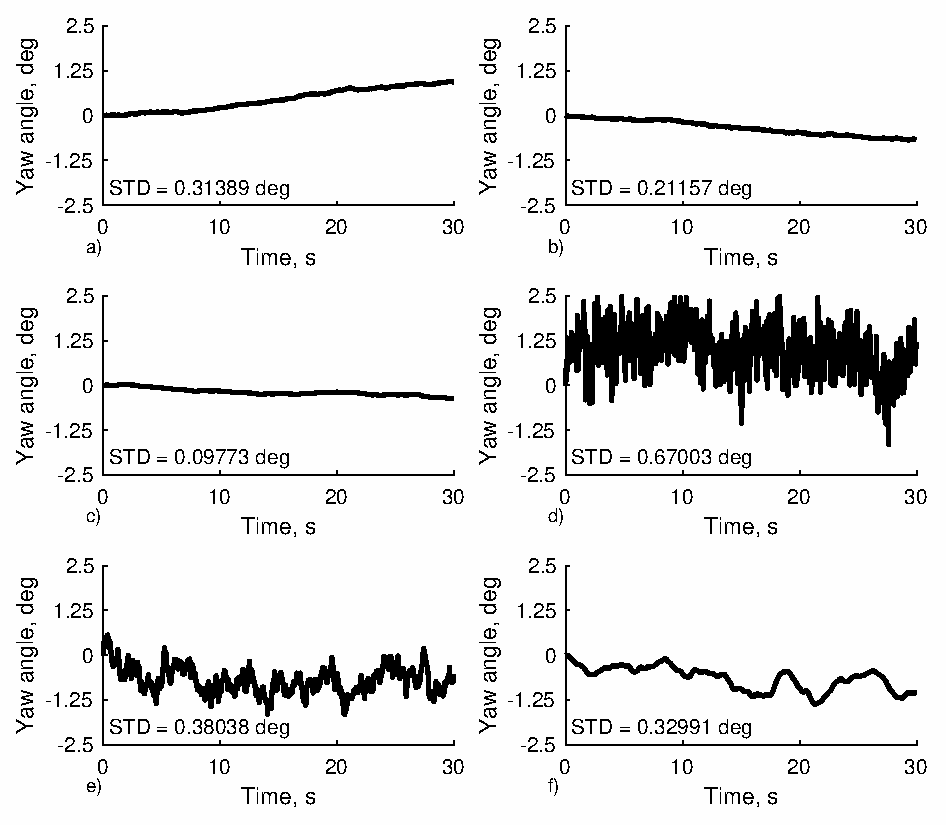
\includegraphics[width=11cm]{IMUbiases.eps}
\caption{Yaw measurements for \textbf{a}) Case 1, \textbf{b}) Case 2, \textbf{c}) Case 3, \textbf{d}) Case 4, \textbf{e}) Case 5, \textbf{f}) Case 6 \label{fig:imubiases}}
\end{figure}
The minimum standard deviation is 0.0973 deg and it is presented for case 3, where only the gyroscope is used, after bias correction and low pass filtering. A angle drift of 0.0124 deg/s is achieved in this case and it is the minimum of all cases. Thus the attitude determination is provided only by the gyroscope data and the low pass filter is given by

\begin{equation}
G_n=(1-f_g) G_{n-1} +f_g G_n^{imu}
\end{equation}
where $G_n$ is the filtered gyroscope value at  $n^{th}$ iteration, $G_n^{imu}$ is the gyroscope measurement provided by the IMU after the bias correction at  $n^{th}$ iteration. $f_g$ denotes the smoothing factor and it is equal to 0.25 for this experimental setup. The loop cycle is selected to be 0.05 s because this is the maximum time period needed to collect the input data from the IMU, execute all the required calculations and write the output data to an SD memory card connected to the native SD Card port of the microcontroller. A flow diagram of the air bearing operation processes that take place is presented in Figure~\ref{fig:start_steps}. 
\begin{figure}[H]
\includegraphics[width=13cm]{startflow.pdf}
\caption{Air bearing operation flow diagram \label{fig:start_steps}}
\end{figure}
At first, the SD card is prepared and a warning message is shown if the initialization has failed. The definition of input, output and interrupt pins follows in order to control the gimbals as presented in the next step. Because of the nature of the encoders, it is possible to achieve only a relative gimbal angle value. This limitations requires the initialization of the gimbals angles to the preferred values in the beginning. Afterwards, the establishment of the $I^2C$ communication takes place that allows to read the data from the IMU and the sensor is calibrated. Eventually, before the beginning of the main operation,  the flywheels are spun up to their operational angular velocity and they are stabilized through a PID controller which remains active through the whole operational time. 

In order to avoid any undesired behaviour, the gimbal rates are saturated according to the following formula:

\begin{equation}
\dot{\boldsymbol{\delta}}_{sat}=\dot{\boldsymbol{\delta}}\hspace{0.1cm}\frac{\dot{{\delta}}_{th}}{\max(|\dot{\delta}_1|,|\dot{\delta}_2|,|\dot{\delta}_3|,|\dot{\delta}_4|)}
\label{eq:saturation}
\end{equation}
where $\dot{{\delta}}_{th}$ is a preset threshold.
It is preferred to saturate the gimbal angle rates using Equation~\ref{eq:saturation} over applying a boundary value to every gimbal angle rate that exceeds the required threshold because the characteristics of the motion are conserved. The saturation threshold is selected to be the minimum value of the maximum gimbal velocity of the four gimbals.
The motor driver takes as input a pulse width modulation (PWM) signal for speed control. Thus, it is required to map each angular velocity of the gimbal to a PWM value, in order to control the CMG cluster. As expected, only an approximation of this is feasible in practice. After achieving the steady state velocity for the four flywheels, each gimbal is spun up gradually by increasing the PWM value while measuring its angular velocity, respectively.  Figure~\ref{fig:degpersec2pwm}a-d shows the relation between the PWM values and the gimbal rates for each CMG.
The equations of the linear approximations that are used to map the commanded gimbal rates to PWM values are also shown in the figure. It is observed that the maximum gimbal velocities are lower than the no-load velocities referred in the datasheet because of the load they support and the fact that they operate at 5V instead of their nominal value of 6V. A cascade control design is implemented and an inner PD controller is used to guarantee that given the commanded gimbal rates, the gimbals follow the desired angle profiles.

\begin{figure}[H]
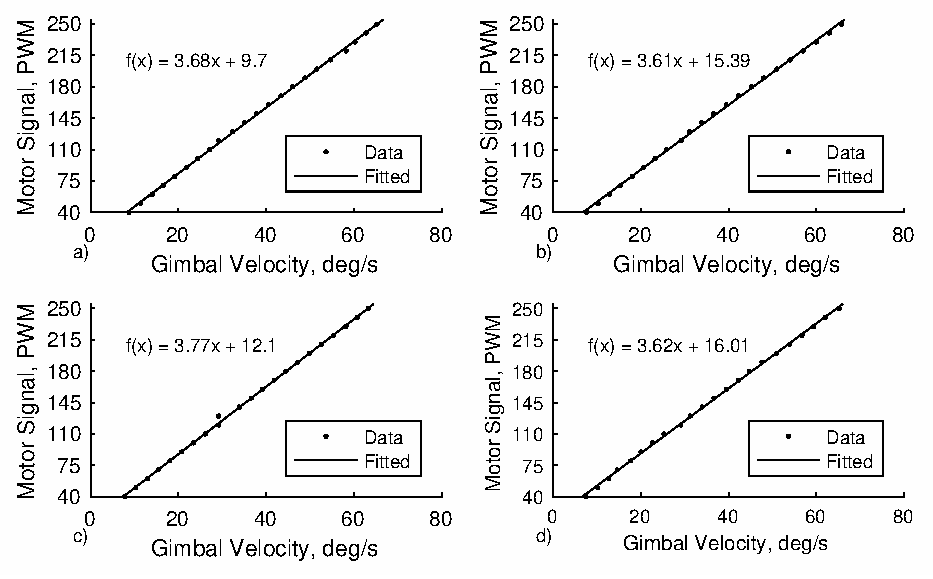
\includegraphics[width=13cm]{degpersec2pwm.eps}
\caption{Deg/s - PWM Relation for \textbf{a}) Gimbal 1, \textbf{b}) Gimbal 2, \textbf{c}) Gimbal 3, \textbf{d}) Gimbal 4 \label{fig:degpersec2pwm}}
\end{figure}


\section{Flywheels - Sizing}
The system is to be tested using an 1 DoF simulator that allows the rotation of the ACS about the yaw axis. A manoeuvre of 30 deg should be completed in 2 s and this requirement is used for sizing the CMG cluster.
Allowing an design error margin, a 2 kg cuboid satellite is selected as reference for sizing. The moment of inertia, $J$, is the same for every axis and it is used to find the required torque, $N_{req}$. This is calculated by:

\begin{equation}
N_{req}=J*\frac{a}{(t_a/2)^2}
\end{equation}
where $a$ is the rotation angle completed in $t_a$ seconds. Figure~\ref{fig:angvel} illustrates the acceleration and deceleration phases of the system.

\begin{figure}[H]
\includegraphics[width=10cm]{wmega_sizing.pdf}
\caption{Angular velocity for rotating $a$ deg in $t_a$ s \label{fig:angvel}}
\end{figure}
The angular momentum $h_{0}$, can be calculated through Equation~\ref{eq:momentum} and following equation:

\begin{equation}
\textbf{N}_{cmg}=\textbf{h}\times \dot{\boldsymbol{\delta}}
\end{equation}
where $\textbf{N}_{cmg} \epsilon {\Re}^{3x1}$ is the total torque generated by the cluster. Due to the symmetric rotation of the gimbals, i.e $\delta_1, \delta_2,\delta_3, \delta_4=\delta$, and assuming that the maximum gimbal velocity, $\delta_{max}$, is the same for all CMGs, the torque for a manoeuvre about the yaw axis is given by 

\begin{equation}
N_{req}=4\dot\delta_{max} h_0 \cos\delta \sin\beta
\end{equation}
For $\delta=0$, the required momentum $h_0$ can be found. This value is used to compute the moment of inertia, $I_f$ through Eq~\ref{eq:h0flywheel}. 

The mass of each flywheel disk, $m_f$ can be easily calculated considering the moment of inertia of the cylindrical tube:

\begin{equation}
m_f=2\frac{I_f}{(z_1^2+z_2^2)}
\end{equation}
for given inner and outer radius $z_1$, $z_2$.
The disks are selected to be 3D printed ABS parts with a known density, $\rho_{abs}$. The mass calculated in the previous step is used to specify the height of the flywheel disks $L_f$, considering the volume of the cylindrical tube as:

\begin{equation}
L_f=\frac{m_f }{\rho_{abs}\pi (z_2^2-z_1^2)}
\end{equation}
The numerical results of the sizing analysis are presented in Table~\ref{table:sizingdetails}
\begin{specialtable}[H] 
\caption{\label{table:sizingdetails} Sizing Details}
%%% \tablesize{} %% You can specify the fontsize here, e.g., \tablesize{\footnotesize}. If commented out \small will be used.
\begin{tabular}{lc}
\toprule
\textbf{Parameter}  & \textbf{Value}   \\
\midrule
$a$                  &   30 deg           \\
$t$                  &   2 s           \\
$J$                &     0.0033 $\mathrm{kgm^2}$            \\
$N_{req}$           &      1.728 mNm \\ %before round 1.7279
$\dot\delta_{max}$        &     35 deg/s  \\
$h_0$             &      0.8661 mNms \\%before round 0.86613
$I_f$             &      0.002068 $\mathrm{gm^2}$ \\%before round 0.0020677
$m_f$           &       14.1 g      \\
$L_f$           &       5.8mm    \\
$\rho_{abs}$          &       2.71 $\mathrm{g/cm^3}$         \\
$z_1$         &         2mm      \\
$z_2$         &         17mm         \\
\bottomrule
\end{tabular}
\end{specialtable}


\section{Dynamic Model}
The equation of motion of a rigid spacecraft is described by:

\begin{equation}
\dot{\boldsymbol{\omega}}=\textbf{J}^{-1}(-\boldsymbol{\omega}\times(\textbf{J}\boldsymbol{\omega})-\dot{\textbf{h}}-\boldsymbol{\omega}\times \textbf{h} + \textbf{T}_{ex})
\label{eq:dyn_eq}
\end{equation}
where $\textbf{T}_{ex} \epsilon { \Re  }^{ 3x1}$ is the vector that contains the external torques applied to the spacecraft and $\boldsymbol{\omega} \epsilon {\Re}^{3x1}$ represents the angular velocity of the spacecraft with respect to the body frame. A control torque, $\textbf{T}_c  \epsilon {\Re}^{3x1}$ can be selected as \cite{lappasthesis}:

\begin{equation}
\dot { \textbf{h} } +\boldsymbol{\omega}\times \textbf{h}=-\textbf{ T }_c
\label{eq:control}
\end{equation}
where $ \textbf{h}\epsilon\Re^{3x1}$ is the angular momentum of the CMG cluster:

\begin{equation}
\textbf{h}=h_0
\begin{bmatrix}
-c\beta s\delta_1-c\delta_2+c\beta s\delta_3+c\delta_4 \\
c\delta_1 -c\beta s\delta_2 -c\delta_3 +c\beta s\delta_4 \\
s\beta s\delta_1+s\beta s\delta_2+s\beta s\delta_3+s\beta s\delta_4
\end{bmatrix}  
\label{eq:momentum}
\end{equation}
$s$, $c$ are the abbreviations for $\sin$ and $\cos$ respectively.  The parameter $\beta$ denotes the skew angle of the 4-CMG cluster in pyramid configuration and it is chosen in such a way that the momentum envelope is nearly 3-axis symmetric and spherical. $h_0$ is the magnitude of the momentum of each flywheel and it is given by:

\begin{equation}
h_0=I_{f}\omega_{f}
\label{eq:h0flywheel}
\end{equation}
where $I_f$ and $\omega_f$ are the moment of inertia and the angular velocity of the flywheel.  

In general, the momentum derived from the CMG cluster is a function of the gimbal angles $\boldsymbol{\delta}=[\delta_1, \delta_2,\delta_3, \delta_4]^T\epsilon\Re^{4x1}$ for a spacecraft employed with 4 CMGs. Assuming that the control torque is known, the relation between the total CMG momentum rate and the gimbal angles rates  can be derived by the equation:

\begin{equation}
   \dot{ \textbf{h}}=\textbf{A}(\boldsymbol{\delta})\dot{\boldsymbol{\delta}}
\end{equation}
The matrix $\textbf{A}(\boldsymbol{\delta})\epsilon\Re^{3x4} $ is the Jacobian matrix of the system and except for the gimbal angles, the Jacobian matrix depends on geometric characteristics of the CMGs like the skew angle. For the 4-CMG cluster the Jacobian matrix is given by:

\begin{equation}
\textbf{A}(\boldsymbol{\delta})=
\begin{bmatrix}
-c\beta c\delta_{1} & s\delta_{2} & c\beta c\delta_{3} & -s\delta_{4}\\
-s\delta_{1} & -c\beta c\delta_{2} & s\delta_{3} & c\beta c\delta_{4}\\
s\beta c\delta_{1} & s\beta c\delta_{2} & s\beta c\delta_{3} & s\beta c\delta_{4}
\end{bmatrix}
\end{equation}
The gimbal angle rate vector $\boldsymbol{\dot{\delta}}\epsilon\Re^{4x1}$ can be calculated by:

\begin{equation}
\label{eq:inverse}
   \dot{\boldsymbol{\delta}}=\textbf{A}^\#(\boldsymbol{\delta}) \dot{ \textbf{h}}
\end{equation}
Since the Jacobian matrix is not rectangular, several definitions have been discussed for the inverse of the Jacobian matrix $\textbf{A}^\#(\boldsymbol{\delta})$ \cite{bongwie2001}.

The satellite's kinematics equation of motion expressed in quaternion form is given by:

\begin{equation}
\dot{\textbf{q}}=\frac{1}{2}\textbf{q}\odot\boldsymbol{\omega}_q
\label{eq:quaternion_dot}
\end{equation}
where $\odot$ denotes the quaternion multiplication and $\textbf{q}=[q_0, q_1, q_2, q_3]^T\epsilon\Re^{4x1}$ represents the attitude quaternion. $\boldsymbol{\omega}_q=[0,\boldsymbol{\omega}^T]^T\epsilon\Re^{4x1}$ is the angular velocity $\boldsymbol{\omega}$ of the satellite expressed in quaternion form. For two quaternions $\textbf{r}=[r_0,r_1,r_2,r_3]^T\epsilon\Re^{4x1}$ and $\textbf{p}=[p_0,p_1,p_2,p_3]^T\epsilon\Re^{4x1}$ the quaternion multiplication is given by:

\begin{equation}
\textbf{r} \odot \textbf{p} =
\begin{bmatrix}
p_0r_0 - p_1r_1 - p_2r_2 - p_3r_3\\
 p_0r_1 + p_1r_0 - p_2r_3 + p_3r_2\\
 p_0r_2 + p_2r_0 + p_1r_3 - p_3r_1\\
 p_0r_3 - p_1r_2 + p_2r_1 + p_3r_0\\
\end{bmatrix}
\end{equation}
For the implementation of the attitude control, the control torque $\textbf{T}_c$ applied on the satellite's body is a function of the vector part of the error quaternion $\textbf{q}_{err}$ and $\boldsymbol{\omega}$ as described by the following equation:

\begin{equation}
\textbf{T}_c=-(K_p\textbf{q}_{err}^v
+K_i\int\textbf{q}_{err}^vdt+K_{\omega}\boldsymbol{\omega})
\end{equation}
The error quaternion between the current attitude quaternion and the commanded quaternion $\textbf{q}^c$ is : 

\begin{equation}
\textbf{q}_{err}=
\begin{bmatrix}
q_{err}^s\\
\textbf{q}_{err}^v
\end{bmatrix}={\textbf{q}^{c}}^{*}\odot\textbf{q}
\end{equation}
where $q_{err}^s$ and $\textbf{q}_{err}^v=[q_{err}^{roll}, q_{err}^{pitch}, q_{err}^{yaw}]^T$ are the scalar and the vector part respectively and ${\textbf{q}^{c}}^{*}$ expresses the conjugate quaternion of $\textbf{q}^c=[q^{c}_0, q^{c}_1, q^{c}_2, q^{c}_3]^T\epsilon\Re^{4x1}$.
The normalization of the quaternions is required before evaluating the $\textbf{q}_{err}$. The "3-2-1" sequence is used to convert the quaternion error to the corresponding Euler angles error as presented in figures in the Simulation Results section.

Since the simulation describes a discrete time system, it is required to integrate the quaternion rate $\dot{\textbf{q}}$ at the $i^{th}$ iteration as given by Equation~\ref{eq:quaternion_dot} using the equation:

\begin{equation}
\textbf{q}_i=\textbf{q}_{i-1}\odot[\cos(||\boldsymbol{\omega}||\frac{dt}{2}), \frac{\boldsymbol{\omega}}{||\boldsymbol{\omega}||}\sin(||\boldsymbol{\omega}||\frac{dt}{2})]^T
\end{equation}
where $dt$ is the time step between two consecutive iterations.

\section{Experimental Setup - Results}
In order to validate the operation of the ACS, two different experiments are conducted. In the first, the platform has to complete an 180 deg manoeuvre about the yaw axis as expressed by the $\textbf{q}^c=[0, 0, 0, 1]^T$. In the second, a 90 deg manoeuvre about the same axis is commanded as given by the quaternion  $\textbf{q}^c=[0.7071, 0, 0, 0.7071]^T$. It is assumed that the system has reached the steady state when the attitude error, $a_{err}$ remains below a preset threshold for a given time $t_{ss}$. The values of the parameters used in the experiments are presented in Table~\ref{table:experimentaldetails}. 

\begin{specialtable}[H] 
\caption{\label{table:experimentaldetails} Experimental Details}
%%% \tablesize{} %% You can specify the fontsize here, e.g., \tablesize{\footnotesize}. If commented out \small will be used.
\begin{tabular}{lc}
\toprule
\textbf{Parameter}  & \textbf{Value}   \\
\midrule
$\beta$         & 54.73  deg              \\
$\omega_f$   & 4000 rpm \\
$K_p, K_i, K_{\omega}$ & 6, 0.001, 6 \\
$\dot{{\delta}}_{th}$         & 64.498 deg/s          \\\ % before round 64.4979
$\boldsymbol{\delta}_{ini}$        & $ [0, 0, 0, 0]^T $ deg \\
$a_{err}$& 1.5 deg \\
$t_{ss}$ & 3 s \\
\bottomrule
\end{tabular}
\end{specialtable}

Figure~\ref{fig:attitude} and Figure~\ref{fig:angles} present the experimental results for the 180 deg manoeuvre. The theoretical data, also shown in each figure, are obtained using the moment of inertia of the system about the vertical axis as measured by the CAD model of Figure~\ref{fig:myACS}a and equals to $J=0.00283$ $\mathrm{kgm^2}$. Figure~\ref{fig:attitude}a illustrates that the system immediately responds to the commanded attitude as it begins to rotate about the positive of yaw the axis. The steady state, as defined previously, is reached at about t=20 s and the rising time of the system is only 3.7 s. This indicates that the platform has gained a high angular velocity as shown also in Figure~\ref{fig:attitude}b. The maximum angular velocity achieved is 53.47 deg/s at t=1.9 s and it follows the theoretical angular velocity profile which presents a maximum value of 51.38 deg/s at t=1.6 s. The mean angular velocity through the whole manoeuvre is 8.32 deg/s. The experimental results differ slightly from the theoretical and a minor time delay is observed in the response due to the low pass filter used to eliminate the sensor noise. However, the system is capable of completing the commanded manoeuvre with an accuracy of 1.5 deg tightly following the theoretical profile.
The gimbal angles of the four CMGs in the cluster are presented in Figure~\ref{fig:angles}a-d respectively. Both minimum and steady state values of each gimbal are shown in Table~\ref{table:gimbalvalues}. The average MAE for this experiment for gimbal angles $\delta_1, \delta_2, \delta_3, \delta_4  $, attitude error and angular velocity as derived by 5 sets of measurements are 4.1654 deg, 4.5314 deg, 7.9983 deg, 15.3848 deg, 3.3122 deg and 1.7429 deg.


\begin{figure}[H]
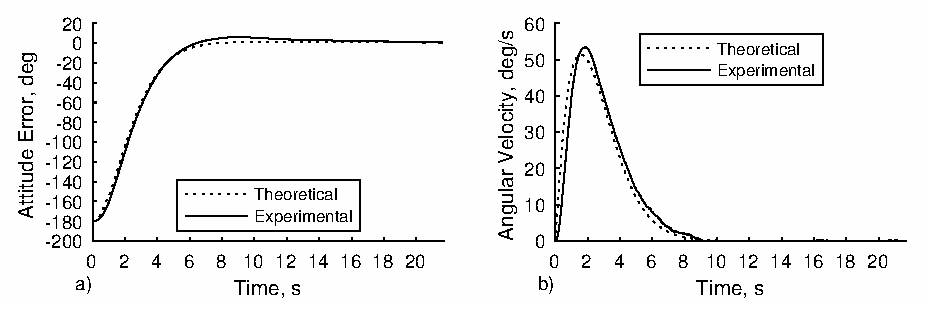
\includegraphics[width=13cm]{attitude.eps}
\caption{\textbf{a}) Attitude error and \textbf{b}) Angular velocity of the platform for 180 deg manoeuvre \label{fig:attitude}}
\end{figure}

\begin{figure}[H]
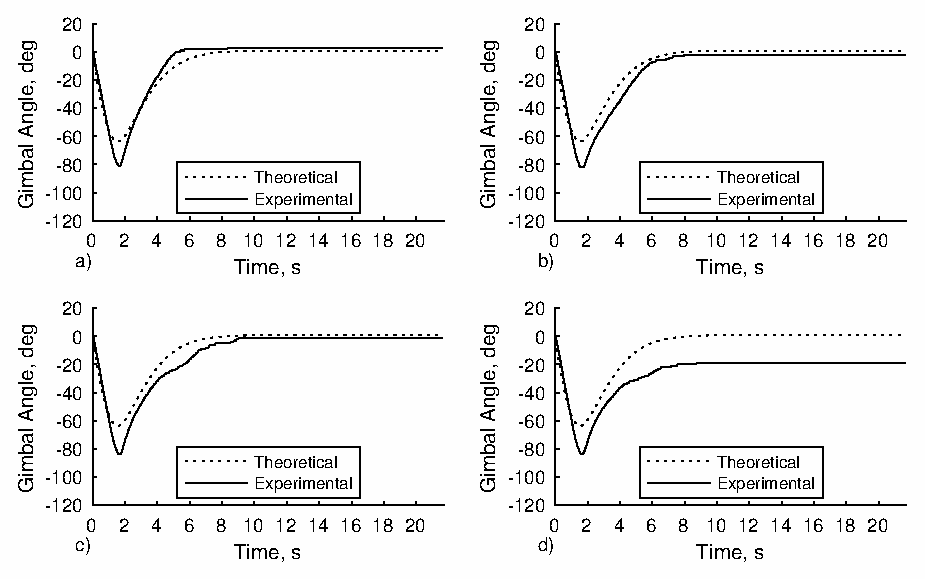
\includegraphics[width=13cm]{angles.eps}
\caption{Gimbal angles for 180 deg manoeuvre, \textbf{a}) $\delta_1$, \textbf{b}) $\delta_2$, \textbf{c}) $\delta_3$, \textbf{d}) $\delta_4$ \label{fig:angles}}
\end{figure}

\begin{specialtable}[H] 
\caption{\label{table:gimbalvalues} 180 deg Manoeuvre - Gimbal angle values}
\begin{tabular}{lc|cc}
\toprule
\multicolumn{2}{l}{\textbf{Parameter} } & \textbf{Theoretical} & \textbf{Experimental}   \\
\midrule
\multirow{2}{*}{$\delta_1$} & Min value                     &-63.7544 deg &  -80.999 deg   \\
                                    & Steady state value       &0.84957 deg & 3.0023 deg      \\
\multirow{2}{*}{$\delta_2$} & Min value                     &-63.7544 deg & -82.0017 deg       \\
                                    & Steady state value      &0.84957 deg  & -1.9996  deg     \\
\multirow{2}{*}{$\delta_3$} & Min value                    &-63.7544 deg  & -84.0013 deg    \\
                                    & Steady state value      &0.84957 deg  & -1.0027  deg     \\
\multirow{2}{*}{$\delta_4$} & Min value                    &-63.7544 deg  & -84.0013 deg        \\
                                    & Steady state value      &0.84957 deg  & -18.9993 deg     \\
\bottomrule
\end{tabular}
\end{specialtable}

Figure~\ref{fig:attitude90} and Figure~\ref{fig:angles90} present the results for the 90 deg manoeuvre. It is observed that the system follows the theoretical attitude and attitude velocity profile as in the previous experiment. A maximum angular velocity of 32.8 deg/s is presented and the platform completes the manoeuvre at about t=17 s. However, the rising time is only 3.25 s while no oscillations are observed, which denotes that the system responds immediately and approaches the desired angle fast. Table~\ref{table:gimbalvalues90} presents the minimum and steady state values of each gimbal. The average MAE for the 90 deg manoeuvre for gimbal angles $\delta_1, \delta_2, \delta_3, \delta_4  $, attitude error and angular velocity as derived by 5 sets of measurements are 12.877 deg, 7.5154 deg, 10.7191 deg,  6.6816 deg, 2.5545 deg and 1.6842 deg.
 

\begin{figure}[H]
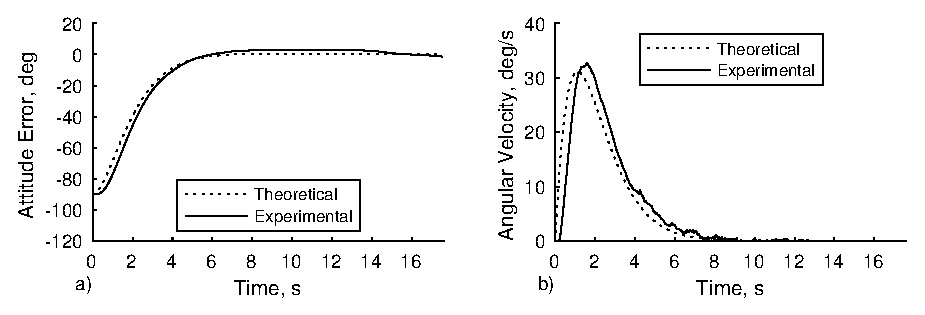
\includegraphics[width=13cm]{attitude90.eps}
\caption{a) Attitude error and b) Angular velocity of the platform for 90 deg manoeuvre \label{fig:attitude90}}
\end{figure}

\begin{figure}[H]
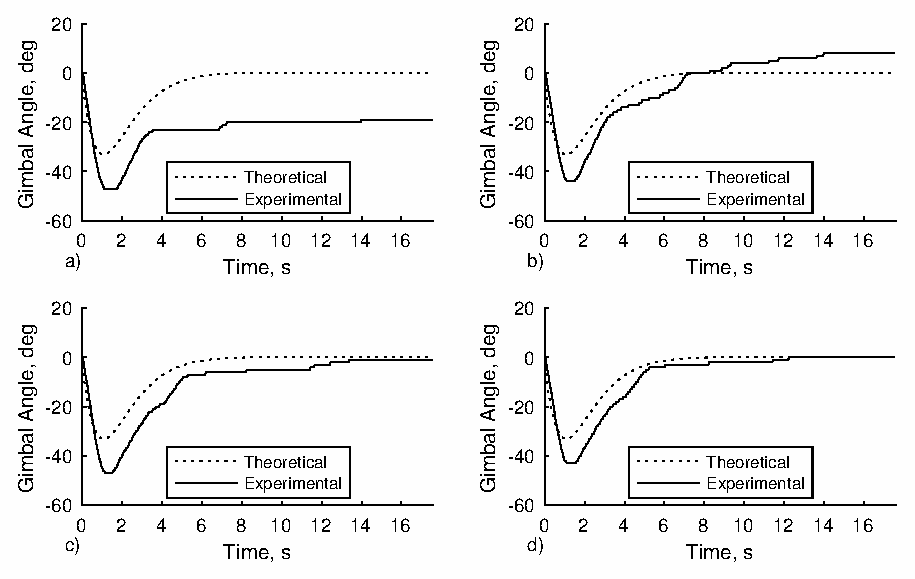
\includegraphics[width=13cm]{angles90.eps}
\caption{Gimbal angles for 90 deg manoeuvre, \textbf{a}) $\delta_1$, \textbf{b}) $\delta_2$, \textbf{c}) $\delta_3$, \textbf{d}) $\delta_4$ \label{fig:angles90}}
\end{figure}

\begin{specialtable}[H] 
\caption{\label{table:gimbalvalues90} 90 deg Manoeuvre - Gimbal angle values}
\begin{tabular}{lc|cc}
\toprule
\multicolumn{2}{l}{\textbf{Parameter} } & \textbf{Theoretical} & \textbf{Experimental}   \\
\midrule
\multirow{2}{*}{$\delta_1$} & Min value                     &-33.1076 deg & - 46.9997 deg   \\
                                    & Steady state value       &0.1761 deg & -18.9993 deg      \\
\multirow{2}{*}{$\delta_2$} & Min value                     &-33.1076 deg & -43.9974 deg       \\
                                    & Steady state value      &0.1761 deg  & 7.9985  deg     \\
\multirow{2}{*}{$\delta_3$} & Min value                    &-33.1076 deg  & -46.9997 deg    \\
                                    & Steady state value      &0.1761 deg  & -1.0027  deg     \\
\multirow{2}{*}{$\delta_4$} & Min value                    &-33.1076 deg  & -43.0005 deg        \\
                                    & Steady state value      &0.1761 deg  & 0 deg     \\
\bottomrule
\end{tabular}
\end{specialtable}


Two main differences are noticed in the gimbal angles profiles of both experiments in comparison to the theoretical profiles. The first is that the minimum values of all four gimbal angles are larger than the expected values. This error is due to various fabrication and assembly imperfections that lead to a non ideal system.
The 3D printed air bearing is naturally introducing a torque error to the rotating platform due to non-zero friction between the upper and the bottom part of the air bearing. In addition, static and dynamic imbalances from flywheels and CMGs along with small torques caused from cables and aerodynamic drag degrade the performance of the air bearing. It has been observed that these manufacturing flaws have a similar effect as increasing the moment of inertia of the rotating platform to $J=0.00323$ $\mathrm{kgm^2}$. The theoretical results obtained this moment of inertia present a better fit to the experimental results for every gimbal in the cluster as well as the angular velocity, compared to the results obtained for the initially estimated moment of inertia of $J=0.00283$ $\mathrm{kgm^2}$. The percentage difference of the MAE values for these two moments of inertia denote that there is a 1.71\% increase only in the first gimbal which is a minor change compared to the decrease in rest of the examined parameters.

\end{paracol}
\nointerlineskip

 \begin{specialtable}[hbtp]
\caption{\label{table:maevalues} MAE values for two different moments of inertia}
\begin{tabular}{lccc}
\toprule
 \textbf{Parameter} &\textbf{MAE for $J=0.00283$ $\mathrm{kgm^2}$}. & \textbf{MAE for $J=0.00323$ $\mathrm{kgm^2}$} & \textbf{MAE - Percentage difference} \\
 \midrule
$\delta_1$     & 3.5261 deg & 3.5863 deg & 1.7073  \%      \\
$\delta_2$     & 4.7112 deg & 3.8116 deg & -19.0949   \%     \\
$\delta_3$     & 4.7787 deg & 4.0325 deg & -15.6151     \%      \\
$\delta_4$     & 18.1385 deg & 17.2076 deg & -5.1322     \%      \\
Attitude error        &  2.4792 deg       &  1.9166 deg      & -22.6928  \% \\
Angular velocity   &  1.5588 deg/s &  1.1199 deg/s & -28.1563   \%\\
\bottomrule
\end{tabular}
\end{specialtable}

\begin{paracol}{2}
\linenumbers
\switchcolumn



The second difference is that steady state value of $\delta_4$ and $\delta_1$ for the first and the second experiment respectively, deviate from the theoretical ones. Positioning the four CMGs in the platform is made manually through 3D printed holes left intentionally for bolt tightening and slight asymmetries may affect the performance of the simulator. Moreover, in the concept of a low cost CMG cluster, the selected gimbal motors present some backlash. In combination with their non-zero stall voltage, a dead zone is admitted for low speeds. As shown also in Figure~\ref{fig:degpersec2pwm}, PWM signals below 40 are considered and handled as zero to prevent the gimbal motors from stalling. These motor imperfections do not affect the flywheel motors since they operate at a constant velocity. Another hardware related limitation is that the gimbals are oriented manually to their initial positions because only relative encoders are employed. Thus, minor misalignments among the initial gimbal angles may provoke the experimental gimbal angles values to deviate from the theoretical ones. 

Despite the limitations discussed above and the extremely low cost of 400 € - 360 € for the electronic components plus 40 € for the 3D printed parts - required to built this attitude simulator,  it has been demonstrated that the system is capable of following efficiently the desired attitude while achieving a high angular velocity which is essential for small and agile satellites. Additionally, that results reveal that CMG cluster rotates the platform significantly faster than it was measured in the sizing process indicating that the design has been made in a very conservative way.
Such angular speeds are critical for Earth observation operations considering that agile spacecrafts aim to capture the larger amount of data possible in a single pass. The cluster presented in this paper points out that it is possible to manufacture a lightweight actuator of small dimensions using COTS components to demonstrate the operation of an agile nano-satellite. It has also been shown that a low cost air bearing with a cost $<$ 400 euros can achieve relatively accurate ($<$ 1.5 deg) performance and can contribute towards the design and testing of new actuators such as CMGs.

Table~\ref{table:cmgscompare} summarises the features of some of the most recent and relevant CMGs proposed for satellites in the micro/nano category along with the characteristics of the CMG presented in this paper.

\end{paracol}
\nointerlineskip

 \begin{specialtable}[H]
\caption{\label{table:cmgscompare} Micro/Nano-satellites with CMGs}
\begin{tabular}{lcccc}
\toprule
 \textbf{Description} &\textbf{ Size, mm} & \textbf{Mass, kg} & \textbf{Max torque, mNm} & \textbf{Max gimbal rate, rad/s} \\
 \midrule
SwampSat \cite{swampsat}    & 100$\times$100$\times$50 & 0.437&0.8 & 57.3\\
Tsubame  \cite{tsubame}  &\diameter50$\times$134 &0.960 &31 & 57.3\\
Lappas  \cite{lappasthesis}  & 150$\times$150$\times$50 &1.170 &52.25 & 11.46\\
Baker \cite{baker}   & 96$\times$96$\times$96& 0.842&1.4 & 600\\
Gaude  \cite{Gaude}  & 100$\times$100$\times$50  &0.250 &1 & 57.3\\ % den exei ylopoihthei omws
Papakonstantinou &178$\times$178$\times$183 & 0.762 & 3.18 & 64.5 \\
\bottomrule
\end{tabular}
\end{specialtable}

\begin{paracol}{2}
\linenumbers
\switchcolumn

The actuator presented in this paper is the largest in size compared to the rest of the CMGs of Table~\ref{table:cmgscompare}. However, its dimensions can be significantly reduced in a real application scenario where the hemispherical piece of the top part of the air bearing is unnecessary and it can be removed. This adjustment could save up to approximately 60 mm along the vertical direction of the actuator. Moreover, it is feasible to further reduce the size of the whole cluster in a future version by positioning the flywheels closer to the gimbals. Selecting or manufacturing smaller slip rings and a tighter configuration of the perfboard along with the battery and the CMGs would also decrease its size.

The CMG cluster presents a maximum torque capability of 3.18 mNm with a maximum gimbal angular velocity of 64.5 rad/s. For the CMGs of the Table~\ref{table:cmgscompare}, only Baker illustrates a higher gimbal rate. However, this is achieved using high-end brushless DC motors by Faulhaber with a cost of nearly 30 times the cost of the gimbal motors utilized in this setup.

% In addition, even though some the CMGs of the Table~\ref{table:cmgscompare} present a higher maximum torque value, the CMG presented in this paper demonstrates significantly higher maximum angular velocity. Table~\ref{table:cmgscomparesvel} illustrates the percentage difference of the maximum velocity of the proposed CMG compared to the CMGs of the Table~\ref{table:cmgscompare}.


% \begin{specialtable}[H]
% \caption{\label{table:cmgscomparesvel} Angular velocity comparison}
% \begin{tabular}{lcccc}
% \toprule
%  \textbf{Description} & \textbf{Max angular velocity} & \textbf{Percentage Difference}  \\
%  \midrule
% SwampSat \cite{swampsat}  & $-$ & $-$  \\
% Tsubame  \cite{tsubame}       &11.46 deg/s  &366.6 \%\\
% Lappas  \cite{lappasthesis}   &8.41 deg/s    &535.8 \%\\
% Baker \cite{baker}                   &3 deg/s         & 1682.3 \%\\
% Gaude  \cite{Gaude}          &1 deg/s         & 5247 \%\\ 
% \bottomrule
% \end{tabular}
% \end{specialtable}
% Moreover, in contrast to the Lappas' CMGs, the proposed CMGs make used of slip rings that allow the 360 deg motion of each flywheel. Baker and Gaude CMG cluster has not yet been implemented and the efficiency of their design has not been evaluated by experimental results.

\section{Conclusion}
An 1 DoF spacecraft attitude control simulator has been designed and manufactured by the Laboratory of Applied Mechanics and Vibrations at the University of Patras. The simulator uses a 4-CMG cluster in pyramid configuration for attitude control and its hardware and software implementation is described in detail. The functionality and the operation of the platform has been evaluated through two different experiments that are validated using single axis manoeuvre theoretical/simulation profiles. It has been demonstrated that despite its low cost and the fabrication imperfections, high manoeuvring capabilities can be achieved utilizing only COTS components and a 3D printed air bearing with a performance better than 1.5 deg (yaw axis). A lot of space remains for improvements. Future work includes the fabrication or the utilization of an enhanced air bearing to improve the  performance of the system, eliminating any undesired friction. The optimization of the configuration and the number of holes used on the bottom part of the air bearings, as well as the material the bearings is made of, can improve the performance of the simulator. In addition, it is feasible to reduce the alignment errors of the gimbals, during the initialization process, using absolute encoders. The absence of an automatic balancing system due to the small size of the whole setup prevents the CMG cluster from exploiting its three dimensional capabilities and it is also reserved for future work. 




%%%%%%%%%%%%%%%%%%%%%%%%%%%%%%%%%%%%%%%%%%


%%%%%%%%%%%%%%%%%%%%%%%%%%%%%%%%%%%%%%%%%%
\vspace{6pt} 

%%%%%%%%%%%%%%%%%%%%%%%%%%%%%%%%%%%%%%%%%%
%% optional
%\supplementary{The following are available online at \linksupplementary{s1}, Figure S1: title, Table S1: title, Video S1: title.}

% Only for the journal Methods and Protocols:
% If you wish to submit a video article, please do so with any other supplementary material.
% \supplementary{The following are available at \linksupplementary{s1}, Figure S1: title, Table S1: title, Video S1: title. A supporting video article is available at doi: link.} 

%%%%%%%%%%%%%%%%%%%%%%%%%%%%%%%%%%%%%%%%%%


\funding{This research received no external funding}

% \dataavailability{In this section, please provide details regarding where data supporting reported results can be found, including links to publicly archived datasets analyzed or generated during the study. Please refer to suggested Data Availability Statements in section ``MDPI Research Data Policies'' at \url{https://www.mdpi.com/ethics}. You might choose to exclude this statement if the study did not report any data.} 

% \acknowledgments{In this section you can acknowledge any support given which is not covered by the author contribution or funding sections. This may include administrative and technical support, or donations in kind (e.g., materials used for experiments).}

\conflictsofinterest{The authors declare no conflict of interest.} 

%% Optional
% \sampleavailability{Samples of the compounds ... are available from the authors.}

%%%%%%%%%%%%%%%%%%%%%%%%%%%%%%%%%%%%%%%%%%
%% Only for journal Encyclopedia
%\entrylink{The Link to this entry published on the encyclopedia platform.}

%%%%%%%%%%%%%%%%%%%%%%%%%%%%%%%%%%%%%%%%%%
% %% Optional
% \abbreviations{The following abbreviations are used in this manuscript:\\

% \noindent 
% \begin{tabular}{@{}ll}
% MDPI & Multidisciplinary Digital Publishing Institute\\
% DOAJ & Directory of open access journals\\
% TLA & Three letter acronym\\
% LD & Linear dichroism
% \end{tabular}}

%%%%%%%%%%%%%%%%%%%%%%%%%%%%%%%%%%%%%%%%%%
%% Optional
% \appendixtitles{no} % Leave argument "no" if all appendix headings stay EMPTY (then no dot is printed after "Appendix A"). If the appendix sections contain a heading then change the argument to "yes".
% \appendixstart
% \appendix
% \section{}
% \subsection{}
% The appendix is an optional section that can contain details and data supplemental to the main text---for example, explanations of experimental details that would disrupt the flow of the main text but nonetheless remain crucial to understanding and reproducing the research shown; figures of replicates for experiments of which representative data are shown in the main text can be added here if brief, or as Supplementary Data. Mathematical proofs of results not central to the paper can be added as an appendix.


% \section{}
% All appendix sections must be cited in the main text. In the appendices, Figures, Tables, etc. should be labeled, starting with ``A''---e.g., Figure A1, Figure A2, etc. 

%%%%%%%%%%%%%%%%%%%%%%%%%%%%%%%%%%%%%%%%%%
\end{paracol}
\reftitle{References}

% Please provide either the correct journal abbreviation (e.g. according to the “List of Title Word Abbreviations” http://www.issn.org/services/online-services/access-to-the-ltwa/) or the full name of the journal.
% Citations and References in Supplementary files are permitted provided that they also appear in the reference list here. 

%=====================================
% References, variant A: external bibliography
%=====================================
\externalbibliography{yes}
\bibliography{mybib}

%=====================================
% References, variant B: internal bibliography
%=====================================
% \begin{thebibliography}{999}
% % Reference 1
% \bibitem[Author1(year)]{ref-journal}
% Author~1, T. The title of the cited article. {\em Journal Abbreviation} {\bf 2008}, {\em 10}, 142--149.
% % Reference 2
% \bibitem[Author2(year)]{ref-book1}
% Author~2, L. The title of the cited contribution. In {\em The Book Title}; Editor1, F., Editor2, A., Eds.; Publishing House: City, Country, 2007; pp. 32--58.
% % Reference 3
% \bibitem[Author3(year)]{ref-book2}
% Author 1, A.; Author 2, B. \textit{Book Title}, 3rd ed.; Publisher: Publisher Location, Country, 2008; pp. 154--196.
% % Reference 4
% \bibitem[Author4(year)]{ref-unpublish}
% Author 1, A.B.; Author 2, C. Title of Unpublished Work. \textit{Abbreviated Journal Name} stage of publication (under review; accepted; in~press).
% % Reference 5
% \bibitem[Author5(year)]{ref-communication}
% Author 1, A.B. (University, City, State, Country); Author 2, C. (Institute, City, State, Country). Personal communication, 2012.
% % Reference 6
% \bibitem[Author6(year)]{ref-proceeding}
% Author 1, A.B.; Author 2, C.D.; Author 3, E.F. Title of Presentation. In Title of the Collected Work (if available), Proceedings of the Name of the Conference, Location of Conference, Country, Date of Conference; Editor 1, Editor 2, Eds. (if available); Publisher: City, Country, Year (if available); Abstract Number (optional), Pagination (optional).
% % Reference 7
% \bibitem[Author7(year)]{ref-thesis}
% Author 1, A.B. Title of Thesis. Level of Thesis, Degree-Granting University, Location of University, Date of Completion.
% % Reference 8
% \bibitem[Author8(year)]{ref-url}
% Title of Site. Available online: URL (accessed on Day Month Year).
% \end{thebibliography}

% If authors have biography, please use the format below
%\section*{Short Biography of Authors}
%\bio
%{\raisebox{-0.35cm}{\includegraphics[width=3.5cm,height=5.3cm,clip,keepaspectratio]{Definitions/author1.pdf}}}
%{\textbf{Firstname Lastname} Biography of first author}
%
%\bio
%{\raisebox{-0.35cm}{\includegraphics[width=3.5cm,height=5.3cm,clip,keepaspectratio]{Definitions/author2.jpg}}}
%{\textbf{Firstname Lastname} Biography of second author}

% The following MDPI journals use author-date citation: Arts, Econometrics, Economies, Genealogy, Humanities, IJFS, JRFM, Laws, Religions, Risks, Social Sciences. For those journals, please follow the formatting guidelines on http://www.mdpi.com/authors/references
% To cite two works by the same author: \citeauthor{ref-journal-1a} (\citeyear{ref-journal-1a}, \citeyear{ref-journal-1b}). This produces: Whittaker (1967, 1975)
% To cite two works by the same author with specific pages: \citeauthor{ref-journal-3a} (\citeyear{ref-journal-3a}, p. 328; \citeyear{ref-journal-3b}, p.475). This produces: Wong (1999, p. 328; 2000, p. 475)

%%%%%%%%%%%%%%%%%%%%%%%%%%%%%%%%%%%%%%%%%%
%% for journal Sci
%\reviewreports{\\
%Reviewer 1 comments and authors’ response\\
%Reviewer 2 comments and authors’ response\\
%Reviewer 3 comments and authors’ response
%}
%%%%%%%%%%%%%%%%%%%%%%%%%%%%%%%%%%%%%%%%%%
\end{document}








